\section{Mini-mundo: modelo E-R para el modelo E-R}

La Figura~\ref{fig:metamodelo-er} conserva el modelo original elaborado por el
equipo. Su propósito es describir los componentes de un modelo E--R y no
representar un mini--mundo externo.

\begin{figure}[htbp]
  \centering
  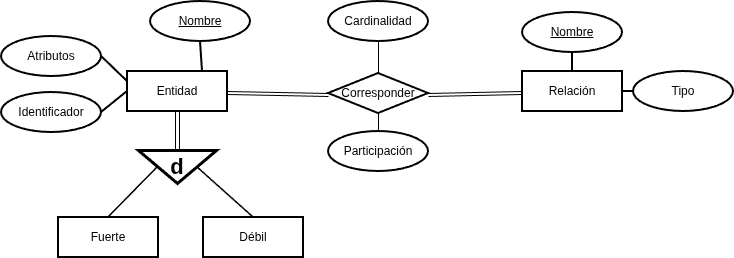
\includegraphics[width=\textwidth]{../Diagramas/Ejercicio3b.drawio.png}
  \caption{Modelo E--R original para los conceptos del propio modelo E--R.}
  \label{fig:metamodelo-er}
\end{figure}

\subsection{Entidades y sus tipos}

\textbf{Entidad} almacena un \emph{Nombre}, sus \emph{Atributos} y su
\emph{Identificador}. La especialización marcada con ``d'' distingue de forma
disjunta los tipos \textbf{Fuerte} y \textbf{Débil}. La línea doble entre
\textbf{Entidad} y el triángulo indica que la clasificación es total: toda
entidad del metamodelo debe pertenecer a uno de esos dos tipos.

El óvalo \emph{Atributos} resume los atributos asociados con la entidad. Sus
características ---simples o compuestos, monovaluados o multivaluados y
almacenados o derivados--- se registran como parte de esa descripción. El
\emph{Identificador} permite señalar los atributos que distinguen a las
instancias; en una entidad débil corresponde a su discriminador junto con la
identidad de la entidad propietaria.

\subsection{Relaciones y restricciones}

\textbf{Relación} posee \emph{Nombre} y \emph{Tipo}. La asociación
\textbf{Corresponder} enlaza entidades con relaciones y permite que una misma
entidad intervenga en diferentes relaciones, así como que una relación reúna
varias entidades. Cuando una entidad participa más de una vez, cada aparición
se interpreta con un papel distinto.

Los atributos \emph{Cardinalidad} y \emph{Participación} pertenecen a
\textbf{Corresponder}, porque describen la intervención de una entidad
específica dentro de una relación. La participación se reconoce gráficamente
con la convención utilizada por el equipo: línea doble para participación total
y línea simple para participación parcial. La cardinalidad se representa con
las flechas de unicidad de la notación vista en clase, sin recurrir a etiquetas
del tipo $1:N$.

El modelo no incorpora herencia ni agregación entre sus conceptos, conforme a
la exclusión indicada expresamente en el enunciado.
